%==============================================================================
% Documentation (pdflatex --interaction=nonstopmode this_file.spad
% Note: ensure that the code above is between \iffalse ... )if false\fi.
%==============================================================================
\documentclass[12pt,a4paper]{article}
\usepackage[utf8]{inputenc}
\usepackage[english]{babel}
\usepackage{amsmath}
\usepackage{amsfonts}
\usepackage{amssymb}
\usepackage{makeidx}
\usepackage{graphicx}
\usepackage{listings}
\usepackage{color}
\usepackage{epstopdf}

\definecolor{dkgreen}{rgb}{0,0.6,0}
\definecolor{gray}{rgb}{0.5,0.5,0.5}
\definecolor{mauve}{rgb}{0.58,0,0.82}
\definecolor{orange}{rgb}{1.0,0.44,0}

\lstdefinelanguage{SPAD}
{keywords={if,then,else,for,in,repeat},
keywords=[2]{Fraction, Integer, Polynomial, Expression, Float, 
             DoubleFloat, SurfaceComplex, CellMap, 
             List},
keywords=[3]{cellMap, bdry, tangentSpace, normalSpace, normalField,
             metricTensor},
keywordstyle=[2]\color{red},
keywordstyle=[3]\color{orange},
sensitive=true,%
alsoletter={\$},%
comment=[l]{--},%
string=[b]",%
string=[b]'%
}

\lstset{frame=tb,
  language=SPAD,
  aboveskip=3mm,
  belowskip=3mm,
  showstringspaces=false,
  columns=flexible,
  basicstyle={\small\ttfamily},
  numbers=none,
  numberstyle=\tiny\color{gray},
  keywordstyle=\color{blue},
  commentstyle=\color{dkgreen},
  stringstyle=\color{mauve},
  breaklines=true,
  breakatwhitespace=true,
  tabsize=3
}
\author{Kurt Pagani \\ {\tt nilqed@gmail.com}}
\date{\today}
\title{SurfaceComplex \\ {\small\tt Domain: SCMPLX}}
%
\newcommand{\CAD}{{\tt CAD}}
\newcommand{\QE}{{\tt QE}}
\newcommand{\RR}[1]{\mathbb{R}^{#1}}
\newcommand{\QQ}[1]{\mathbb{Q}^{#1}}
\newcommand{\ZZ}[1]{\mathbb{Z}^{#1}}
\newcommand{\KK}[1]{\mathbb{K}^{#1}}
%
\begin{document}
\maketitle
%
\begin{abstract}
This manual decribes the FriCAS domains {\bf CellMap} and 
{\bf SurfaceComplex}. These domains provide methods to compute
various differential geometric objects of so called $p$-surfaces
in ${\RR n}$, a notion which is used by Walter Rudin in his famous
{\it Principles of Mathematical Analysis}. 
\end{abstract}
%
\section{Introduction}
%
Dealing with manifolds or similar geometric structures in a scientific
computing system like FriCAS requires a great deal of abstraction as well
as some simplifications compared to the usual mathematical definitions of
such objects. It makes not much sense to speak of open sets, charts,
diffeomorphisms and other topological properties in this context. Of 
course, it is not impossible to mimic such terms in FriCAS, however,
it would be of little use since most of them were not computable
anyway. Since we already have differential forms and jet bundles at
hand, we are looking for {\it dual} objects, so that we will be able
to integrate differential forms over {\it surfaces} for example, that
is to have some form of {\em Stokes theorem}:
\begin{displaymath}
  \int_{M} d\,\omega = \int_{\partial M} \omega
\end{displaymath}   
The identity above holds for a wide range of objects $M$ and $\omega$,
and is - roughly speaking - the basis of geometric integration 
\cite{GIT} and/or geometric measure theory \cite{GMT}. The generalization
of Stokes theorem in those theories looks like
\begin{displaymath}
    \langle M,d\, \omega\rangle = \langle \partial M, \omega \rangle,
\end{displaymath}  
where the pairing $\langle\cdot,\cdot\rangle$ usually denotes a bilinear
mapping between so called {\em chains} and {\em co-chains}. In the 
approach \cite{GIT} by Whitney (and recently by Harrison \cite{JH}) the
chains $M$ are built by geometric primitives (e.g. polyhedral chains)
forming normed linear spaces (for various norms like {\em sharp} or
{\em flat}) whose duals are the corresponding Banach space of co-chains,
where it is not clear a priori that they represent differential forms 
(this can be shown under certain conditions and is a highly non-trivial
task). The other approach (as described by Federer \cite{GMT}) starts
from smooth differential forms and looks at the dual space, well known
as {\em DeRham Currents}. The whole theory is more or less a fruitful
generalization of Laurent Schwartz's concept of {\em distributions}.
In this context Stokes theorem holds by definition:
\begin{displaymath}
      T(d\,\omega) = \partial T (\omega),
\end{displaymath}
for all smooth forms and all currents (comparable to the derivatives
of distributions $T'(\varphi)=-T(\varphi')$). This means $\partial$ is
a linear operator (usually called {\em boundary operator}) which is
loosely speaking the transpose of the differential operator $d$.

Here we will follow along the lines of the latter approach, that is we
are going to deal with objects which might be seen as DeRham currents
in a wider sense, though we only consider {\em nice} objects (currents
form a really huge space and many elements look quite bizarre) which
have some relation to differential geometry.



\begin{lstlisting}
 -- code
\end{lstlisting}

%
%\begin{figure}[!htb]
%\centering
%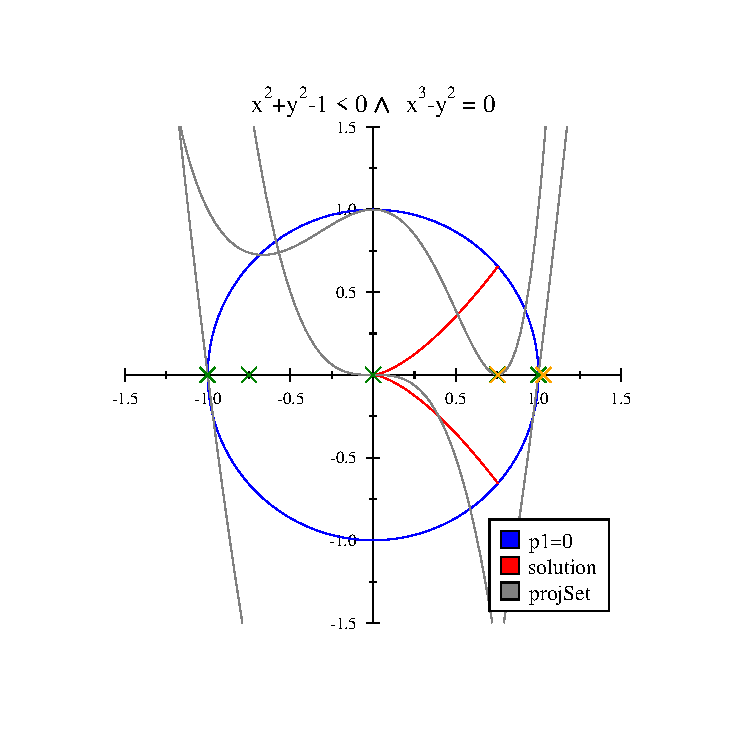
\includegraphics[scale=1.0]{cad1.eps}
%\caption{Example 1.}
%\label{fig:cad1}
%\end{figure}
% 
\begin{thebibliography}{1}
%
\bibitem{rudin1976principles} Walter Rudin,
  {\em Principles of Mathematical Analysis},
  International series in pure and applied mathematics,
  1976, McGraw-Hill.
\bibitem{GIT} Hassler Whitney. {\em Geometric Integration Theory},
  Princeton Mathematical Series, No. 21. Literary Licensing, LLC.
\bibitem{GMT} Herbert Federer. {\em Geometric Measure Theory}. Springer,        
  Reprint of the 1st ed. Berlin, Heidelberg, New York 1969 edition.
\bibitem{JH} Jenny Harrison, {\em Operator Calculus of Differential
  Chains and Differential Forms}, to appear in the Journal of Geometric
  Analysis, 2013. \\
  Url:\ {\small {\tt math.berkeley.edu/\textasciitilde harrison}}
\end{thebibliography}
%
\end{document}
% -----------------------------------------------------------------------------
% END DOCUMENTATION
% -----------------------------------------------------------------------------